\documentclass[table]{beamer}
\mode<presentation>
\usetheme{Berlin}
\usecolortheme{beaver}
\usepackage{listings}
\usepackage{multirow}

%%%
% TITLE PREAMBLE
\title[Intro to Bioinformatics] % (optional, only for long titles)
{An Introduction to Bioinformatics Tools}
\subtitle{Part 2: BLAST}
\author[Pritchard, Cock] % (optional, for multiple authors)
{Leighton~Pritchard \and Peter~Cock}
\institute[The James Hutton Institute] % (optional)
{
  Information and Computational Sciences\\
  The James Hutton Institute
}
\date[May 2014] % (optional)
{Bioinformatics Training, 29$^{th}$ May 2014}
\subject{Bioinformatics}

%%%
% TOC
% Show table of contents, with current section highlighted,
% at the start of each section
\AtBeginSection[]
{
  \begin{frame}
    \frametitle{Table of Contents}
    \tableofcontents[currentsection]
  \end{frame}
}


%%%
% START DOCUMENT
\begin{document}

  \frame[plain]{\titlepage}
  
%%%
% SECTION: BLAST Essentials
  \section{BLAST Essentials}
  
    % What is BLAST
    \subsection{What is BLAST?}
    \begin{frame}
     \frametitle{What BLAST Is}
     \begin{itemize}
       \item Basic (it's actually sophisticated)
       \item Local Alignment (what it does: local sequence alignment)
       \item Search Tool (what it does: search against a database)
       \item The most important software package in bioinformatics?
       \item Fast, robust, sequence similarity search tool
       \item Not foolproof.
     \end{itemize}
    \end{frame}
  
    \begin{frame}
     \frametitle{What A BLAST Search Is}
     \begin{itemize}
       \item BLAST search = identification of similar sequences in a database
       \item This depends on:
       \begin{itemize}
         \item query sequence
         \item BLAST program (and choice of BLAST/BLAST+, version No.)
         \item database
         \item search parameters
       \end{itemize}
     \end{itemize}
    \end{frame}  
  
    % How BLAST works
    \subsection{How BLAST works}
    \begin{frame}
     \frametitle{Assumptions}
     You are familiar with
     \begin{itemize}
       \item biological sequences (RNA, DNA, protein)
       \item mutation, drift, molecular clocks
       \item gene and genome structure (including repeats, pseudogenes etc.)
       \item homology, paralogy, orthology, etc.
     \end{itemize}
     - important for interpretation of BLAST output
    \end{frame}
    
    \begin{frame}
      \frametitle{High-level Overview}
    \end{frame}

    \begin{frame}
     \frametitle{Global \textit{vs} Local Alignment}
     \begin{itemize}
       \item<1-> Global alignment: sequences are aligned along their entire lengths
       \item<1-> Local alignment: the best subsequence alignment is found
       \item<2-> Consider an alignment of the same gene from two distantly-related eukaryotes, where:
         \begin{itemize}
           \item<2-> Exons are conserved and small in relation to gene locus size
           \item<2-> Introns are not well-conserved but large in relation to gene locus size
         \end{itemize}
       \item<3-> Local alignment will align the conserved exon regions
       \item<3-> Global alignment will attempt to align mostly unrelated sequence
     \end{itemize}
    \end{frame}

    \begin{frame}
     \frametitle{Dynamic Programming}
     \begin{itemize}
       \item<1-> We aim to align the words
       \begin{itemize}
         \item<1-> \texttt{COELACANTH}
         \item<1-> \texttt{PELICAN}
       \end{itemize}
       \item<2-> Each identical letter (match) scores +1
       \item<2-> Each different letter (mismatch) scores -1
       \item<2-> Each gap scores -1
       \item<3-> How do we maximise the alignment score?
     \end{itemize}
    \end{frame}   
   
    \begin{frame}
     \frametitle{Dynamic Programming}
     \framesubtitle{Initialise the matrix}
       \begin{center}
         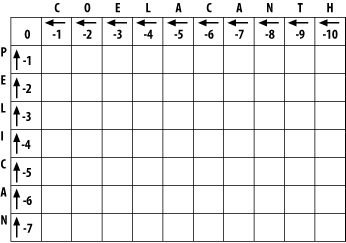
\includegraphics[width=0.5\textwidth]{images/initialise}
       \end{center}
    \end{frame}   
   
    \begin{frame}
     \frametitle{Dynamic Programming}
     \framesubtitle{Fill the cells}
       \begin{center}
         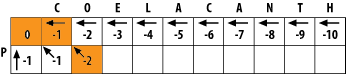
\includegraphics[width=0.5\textwidth]{images/fill_start} \\
         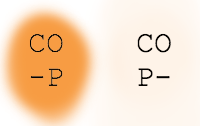
\includegraphics[width=0.3\textwidth]{images/fill_start_letters}
       \end{center}
    \end{frame}     

    \begin{frame}
     \frametitle{Dynamic Programming}
     \framesubtitle{Fill the matrix}
       \begin{center}
         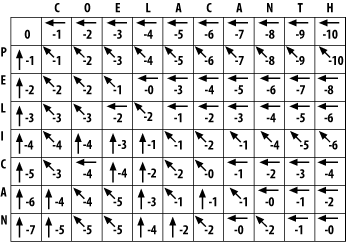
\includegraphics[width=0.5\textwidth]{images/full_matrix}
       \end{center}
    \end{frame}  
   
    \begin{frame}
     \frametitle{Dynamic Programming}
     \framesubtitle{Traceback}
       \begin{center}
         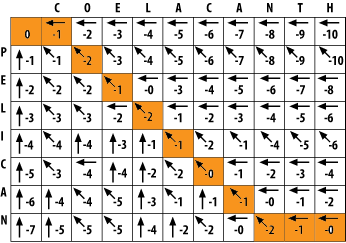
\includegraphics[width=0.5\textwidth]{images/traceback} \\
         
\includegraphics[width=0.3\textwidth]{images/traceback_sequence}         
       \end{center}
    \end{frame}     

    \begin{frame}
     \frametitle{Dynamic Programming}
     \framesubtitle{Algorithms}
       \begin{itemize}
         \item<1-> Global: Needleman-Wunsch (as in example)
         \item<1-> Local: Smith-Waterman (differs from example)
         \item<2-> NW/SW are \emph{guaranteed} to find the optimal match \emph{with respect to the scoring system begin used}.
         \item<3-> BLAST doesn't use these algorithms, which is one reason why it's fast.
       \end{itemize}
    \end{frame}   

    \begin{frame}
     \frametitle{Dynamic Programming}
     \framesubtitle{Gap Scoring}
       \begin{itemize}
         \item Simple gap penalty: all gaps score the same
         \item Affine gap penalty: opening and extending score differently
       \end{itemize}
    \end{frame}  
   
  \section{Using BLAST}
    \subsection{Which BLAST tool should I use?}
    \begin{frame}
     \frametitle{}
    \end{frame}

    \subsection{Controlling BLAST output}
    \begin{frame}
     \frametitle{}
    \end{frame}
     
    \subsection{Interpreting BLAST output}
    \begin{frame}
     \frametitle{}
    \end{frame}
    
% etc
\end{document}